%%%%%%%%%%%%%%%%%%%%%%%%%%%%%%%%%%%%%%%%%%%%%%%%%%%%%%%%%%%%%%%%%%%
%% chapter1.tex
%% UNL thesis document file
%%
%% Chapter with introduction
%%%%%%%%%%%%%%%%%%%%%%%%%%%%%%%%%%%%%%%%%%%%%%%%%%%%%%%%%%%%%%%%%%%
\newcommand{\unlthesis}{\emph{unlthesis}}
\newcommand{\unlthesisclass}{\texttt{unlthesis.cls}}


\chapter{Introduction}
\label{cha:introduction}

\section{Context}

Although during conversations major attention is given to the spoken content, non-verbal communication processing occurs subconsciously. Besides the verbal content of speech, it contains also non-verbal elements known as paralanguage: voice quality, rate, pitch, volume, and speaking style, prosodic features such as rhythm, intonation, and stress. But there are additional visual cues part of the non-verbal communication, namely, body language (kinesics), distance (proxemics), oculesics (eye contact, patterns of fixation, etc.), and touch (haptics). Together with paralanguage, non-verbal communication make two thirds of communication \cite{Burgoon2016}.

As such an important part of communication is visual, the goal of this thesis is to collect RGB and depth video data related to communication, analyze and detect different communication features by applying image processing techniques as well as machine learning. For that purpose different study cases have been carefully selected:
\begin{enumerate}
    \item \textbf{Speech and Language Therapy}: evaluation of oromotoric exercises performed by children with lisp problems in context of the project BioVisualSpeech.
    \item \textbf{Affective computing}: detecting and recognizing emotional states of humans.
    \item \textbf{Facial paralysis}: detect and quantify the severity of facial paralysis \cite{Ngo2016}\cite{Sundaraj2012}.
\end{enumerate}

Study case 1) is part of an international project called BioVisualSpeech in which this thesis is part of. In Fig.\ref{fig:project} an overview of the project, which aims to collect data from children with speech disorders, is provided. The project is composed by three main components: a) data acquisition using interactive games, b) Data analysis, and c) health information system. The goal of BioVisualSpeech is to develop a system that is composed by the three mentioned components in order to support speech therapists (more details in chapter \ref{sec:motivation}). During this thesis the focus lies on RGB and depth video processing, annotation extraction and development of a system which uses machine learning techniques to find similar patients and suggest therapy exercises. 

\begin{figure}
    \centering
    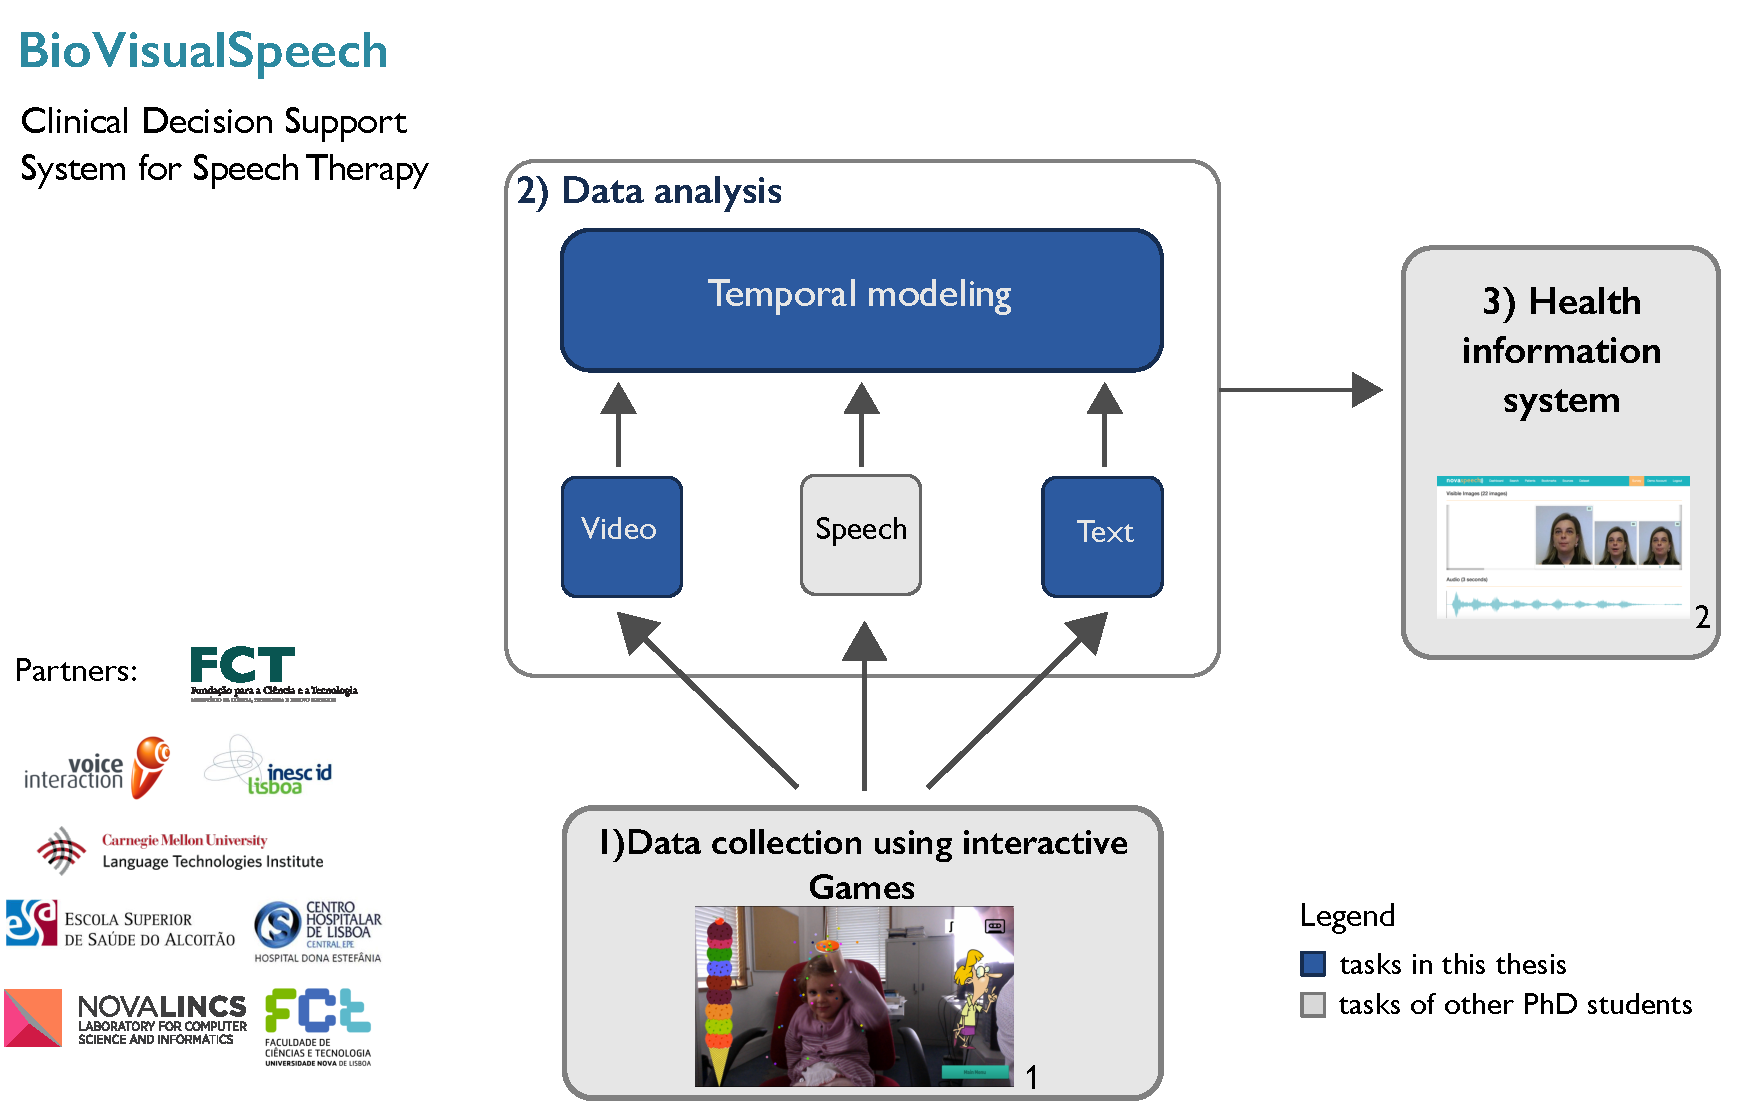
\includegraphics[width=13cm]{diagramProject.pdf}
    \caption{Overview of the project BioVisualSpeech.}
    \label{fig:project}
\end{figure}

Study case 2) was chosen as several datasets for expression detection are available and a taxonomy for facial movements is available in this area. As in study case 1) also facial movements have to be extracted and represented, the goal is to learn the state-of-the-art in expression detection in order to apply it to study case 1).

Study case 3) is similar to study case 1) with the difference that there is no pathology concerning speech. However, neurological diseases can cause facial paralysis which are visible and which disturb speech production and non-verbal communication. Through physiotherapy during several weeks, the gravity of the paralysis can be reduced. 

All three study cases have in common the video analysis of facial activity over a temporal window and it is expected that the same image processing and machine learning tools can be applied. In the following subchapters the motivation and impact will be described.  



% ==================================================================

\section{Motivation} % (fold)
\label{sec:motivation}

The human face can provide several insights such as the emotional state, symptoms of diseases (pain, elevated blood pressure, facial paralysis, autism etc.), engagement in a conversation, and so on. However, the given examples are difficult to measure quantitatively and are mainly subjective.\\

In 1995, Rosalind Picard first published the term affective computing which has become a growing interdisciplinary research area in the last years. The area started by the curiosity to measure the emotional state of study participants quantitatively instead of being measured by questionnaires through self-reporting \cite{Picard2014promise}. Detection and understanding of human affects have become important not only in human-computer interaction but also in areas such as medicine, literature, psychology, and marketing.\\

Such as the human face musculature is important to express feelings and the interior state of mind, it is also essential for verbal communication. Understanding facial activity during speech could help improve speech analysis when speech recording has poor quality or is not present. Additionaly, by knowing how facial muscles are engaged during speech, dysfunction and its severity could be detected. Understanding the tools used for facial expression detection in order to apply them to health domains such as speech therapy is one of the main goals of this thesis.

And why speech therapy? In the year 2000, 40 million Americans had communication disorders causing a cost to the U.S. of approximately \$154-186 billion anually which was equal to 2.5-3\% of the Gross National Product \cite{Ruben2000}. The U.S. employment market has become more and more dependent on communication skills (hearing, voice, speech, and language) as in several industries manual work is being automated. And although it might seem that hearing loss brings more economic disadvantage than the lack of another communication skill, people with severe speech disabilities are more often unemployed or in a lower economic class \cite{Ruben2000}.

In order to reduce prevalence of speech disorders, it is essential to detect and treat speech disabilities as soon as possible, considering that 5\% of US children aged 3-17 years have a  speech disorder, which means that they have difficulties in producing sounds of speech and problems with the quality of voice \cite{SpeechStatistics}. Supporting speech and language therapists (SLTs) in that task is the purpose of the project BioVisualSpeech. The goal of this project is to develop a system that provides SLTs with exercises incorporated in interactive games and an information system that enables therapists to easily review the exercise performance of their patients through video recordings. The main goal however, is to develop a machine learning system that analyzes the data collected during the games and recognizes patterns using data of other patients in order to extract new insights and suggest exercises that suit the learning progress of the patient.  

The same setting could also be applied to patients with facial paralysis, caused by nerve damage. It usually occurs on only one side of the face and can have different degrees of severity which cause difficulty not only in speaking but also in eating and drinking. Although there are more than twenty grading methods of the severity of facial paralysis, they have defaults in integration, feasibility, accuracy, and reliability \cite{Dong2008}. The development of an accurate method for detection and grading of facial paralysis based on image processing would be beneficial to clinicians and patients.


For both, speech therapy and facial paralysis therapy, treatment takes several months of therapy sessions in which various exercises are performed to improve weakness in oral musculature. The video monitoring during therapy combined with the analysis of face muscle performance could help therapists to follow up the progress of each patient, compare patients with similar problems and even provide therapists with quantitative measurements. The inclusion of affective computing in the face analysis system, would accquire additional information of the patient's degree of engagement during the exercises being an additional factor to a successful therapy. Through the use of different sources of data such as health records, a multimodal time series of observations is used to develop a clinical decision support system that supports therapists in providing personalized therapies.
% ==================================================================

\section{Challenges and Impact}

A Clinical Decision Support for SLTs would be a valuable additional tool as it would suggest therapists next exercises for the patient based on his/her progress and those of patients with similar problems. Through the availability of multimodal data, new insights can be gained to develop and improve personalized therapies. By analyzing the therapy progress and comparing it with those of patients with similar problems and learning rate, the therapy length could be predicted which is an interesting information for the therapist.
2) impact of emotional state of the patient can be taken into account and explain fast/slow progress.\\

\textbf{Long-term vision- How to provide SLTs with exercises suggestions based on the analysis of the patient history and previous knowledge?} More details after writing state-of-the-art.

To fullfil this vision I shall address two research challenges:

\textbf{Challenge 1- Relate facial muscle activity to speech (Portuguese and/or U.S. English) using RGB, depth and infrared video data.}
In the literature, to the best knowledge of the writer, databases with all three modalities recording speech exercises were not found. Besides obtaining/creating such a data set, the biggest challenge will be to develop image processing features that are robust to different light conditions, background, skin color and age of the patient. Additonally, a machine learning algorithm needs to be found that can map facial activity to speech production (study case 1) and degree of facial paralysis (study case 3).

\textbf{Impact 1}
New insights of speech disorders can be obtained, as well as quantitative measures which in speech therapy and in the diagnoses of facial paralysis are currently are not sufficiently feasible. Besides that, the creation of a visual database would enable the therapist to review the progress of the therapy visually and not just with text annotations. \\

\textbf{Challenge 2- Mathematical representation of different modalities and temporal information.} More details after writing state-of-the-art. \\

\textbf{Impact 2} A feature space that can represent the progress of different measurements over time can be used in several applications. More details after writing state-of-the-art.\\

% ==================================================================


\section{Research hypotheses}

The goal of this thesis is to analyze facial activity, produced by speech therapy exercises and facial paralysis exercises, recorded by RGB, depth, and infrared cameras during several therapy sessions in order to develop a clinical decision support system that uses multimodal data to support health professionals in their decisions through exercise suggestions.

As seen in Fig.~\ref{fig:project}, the scope of this work is limited on exploring feature representations for video data and introducing text information into the machine learning framework, which is also part of this thesis, in order to represent progress done by the patient on different time instants (temporal modeling). In the following, the milestones to reach the goal of this thesis will be presented and explained. \\

Link this to a Gantt chart.

\textbf{Task 1- Research image features for RGB, depth, and infrared data that permit the mapping of visible facial muscle activity to correct/incorrect execution of speech exercises OR paralysis severity.} It is expected that by combining different modalities (RGB, depth, infrared) the feature representation of facial activity is improved. The goal is that the feature representation permits the binary classification of correct/incorrect execution of speech exercises in the case of applying to speech therapy. In the case of facial paralysis the goal is to have a feature representation that permits a multiclass classification for the degree of severity of the paralysis.\\

\textbf{Task 2 - Understand the relation ... engagement during exercises through detecting relevant facial expressions.} Speech therapy requires monotonous repetition of exercises which can affect the engagement of the patient. By detecting in real-time the disengagement of the patient, different exercises can be suggested to maintain a positive learning curve. \\

\textbf{Task 3 - Research feature spaces that relates in meaningfully manner information from different modalities, therapist annotations and time.}
Suuport the SLTs reasoning and exploration of health data. 
Additionally to visual features, therapist annotations will be used to represent the progress of the therapy over time. As the therapy is performed through several sessions the time component is essential to measure the progress of a patient. 

\textbf{Task 4 - Develop statistical model that suggests future exercises by comparing one patient with similar ones in an existing database.} By being able to model the temporal progress of the therapy, the progress of one patient can be compared to the progress of others. Patients with similar starting point and positive conclusion of the therapy, can be taken as example and can provide insights of therapeutic actions that can help other similar patients to improve their progress. Thus, future actions to take can be suggested to the therapist. This model could also be used for other applications where temporal progression of a disease is observed through several therapy sessions.  

\begin{comment}
Considering clinical medical data existing in the Electronic Health Records, in particular, multimodal time series of data from health sensors and medical notes collected at each patient visit, we wish to recognize health/clinical patterns to support health professionals in their decisions through (i) suggestions and (ii) similar examples.
\end{comment}

\section{Contributions}

Since September 2016 the following contributions have been made.
\begin{enumerate}
\item Collection of a new 3D video dataset recorded with a Microsoft Kinect 2,  containing oro-facial motor exercises performed by children of the age ... with no prior speech disorder diagnosis 
\item Benchmark of embeddings for facial representation
\item Survey of state-of-the-art in expression detection and image processing for facial paralysis detection
\end{enumerate} 



